%\documentclass{article}
%\usepackage{amsmath}
%\usepackage{graphicx}
%\usepackage{tikz}

%\begin{document}

%\section*{Objectives}

The purpose of this experiment is to accurately determine the charge-to-mass ratio \( \frac{e}{m} \) for an electron by observing and analyzing the behavior of electrons accelerated under controlled electric and magnetic fields. Electrons are emitted from a heated filament by thermionic emission and subsequently accelerated by a known potential difference \( \Delta V \). This energy provides the electrons with a specific kinetic energy, allowing them to enter the magnetic field generated by a pair of Helmholtz coils with a known and uniform magnetic induction \( B \). 

Within this magnetic field, electrons are subjected to the Lorentz force, which causes them to follow a circular trajectory due to the perpendicular orientation of their velocity relative to the field \( B \). The radius of this trajectory is directly influenced by the balance between the centripetal force and the magnetic force acting on the electrons. By systematically varying \( \Delta V \) and the current \( I \) in the Helmholtz coils, the experiment allows for precise measurements of the trajectory radius, enabling calculation of the \( \frac{e}{m} \) ratio from macroscopic variables.
Additionally, this experiment measures the horizontal component of Earth’s magnetic field by observing deflections of a magnetic needle at different currents. This measurement helps account for Earth’s magnetic influence, enhancing the accuracy of electron dynamics analysis in combined electric and magnetic fields. Measurements are performed in multiple orientations to assess the effect of Earth’s horizontal magnetic field component on the electron trajectory. The setup includes configurations in which the magnetic field of the coils is first orthogonal, then parallel, and finally antiparallel to Earth’s magnetic field.

Errors are minimized by adjusting the setup's orientation and correcting Earth’s magnetic field measurements with a magnetic needle. A mirror behind the setup reduces parallax errors when measuring the electron beam's diameter. Adjusting voltage and current stabilizes the beam's path diameter, improving measurement consistency.

This experiment effectively determines the electron’s charge-to-mass ratio by linking electric and magnetic measurements to calculate its circular motion under controlled conditions.

\begin{figure}[h!]
    \centering
    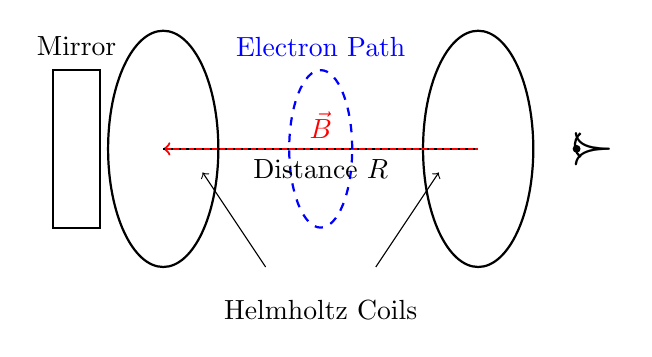
\begin{tikzpicture}
        % Helmholtz Coils 
        \draw[thick] (-2,0) ellipse (0.7cm and 1.5cm);  % Left coil
        \draw[thick] (2,0) ellipse (0.7cm and 1.5cm);   % Right coil

        % Magnetic Field 
        \draw[->, thick, red] (2,0) -- (-2,0) node[midway, above] {$\vec{B}$};

        % Electron Path 
        \draw[blue, thick, dashed] (0,0) ellipse (0.4cm and 1cm);
        \node[blue] at (0,1.3) {Electron Path};

        % Distance R between coils
        \draw[thick, dotted] (-2,0) -- (2,0) node[midway, below] {Distance $R$};

        % Mirror
        \draw[thick] (-3.4,-1.0) rectangle (-2.8,1.0);
        \node at (-3.1,1.3) {Mirror};

        % Helmholtz coils label
        \node[below] at (0,-1.8) {Helmholtz Coils};
        \draw[->] (-0.7,-1.5) -- (-1.5,-0.3);
        \draw[->] (0.7,-1.5) -- (1.5,-0.3);

                   % Eye 
        \node at (3.45, 0) {\huge \textbf{\(\succ\)}}; % weird symbol
        \draw[thick] (3.3,0.2) arc[start angle=130, end angle=230, radius=0.2cm]; % curved part from 130 to 230 degrees
        \fill[black] (3.25,0) circle (0.05); % point


    \end{tikzpicture}
    \caption{Schematic of the Experimental Setup with Helmholtz Coils}
    \label{fig:setup}
\end{figure}


%\end{document}
